

\chapter{Stream Ciphers}	
	
	\begin{definition}[Stream Ciphers]\ 
	    \begin{itemize}
	        \item Basic Idea: Take a short key, expand it into a long key and use as one-time pad.
	    \end{itemize}
		\begin{center}
			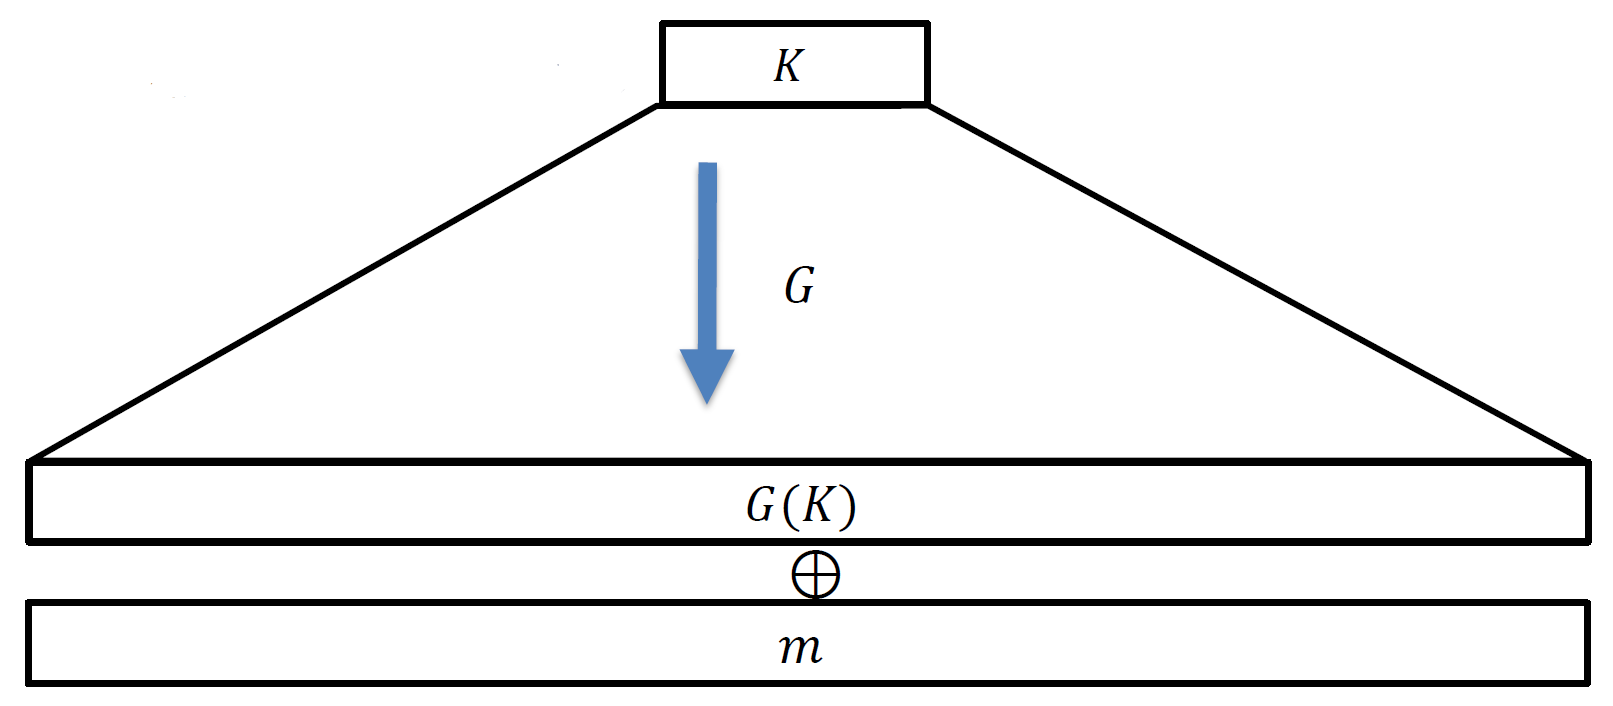
\includegraphics[width=120mm]{Graphics/Basics of Private Key Encryption/StreamCiphers.png}\newline
		\end{center}
		\begin{itemize}
	        \item $KeyGen(1^{\lambda})$: Choose $K \leftarrow_{\$} \{0,1\}^{\lambda}$, output $K$
	        \item $Enc(K,m)$: Compute and output $c \leftarrow G(K) \oplus m$
	        \item $Dec(K,m)$: Compute and output $m \leftarrow G(K) \oplus c$
		\end{itemize}
	\end{definition}
	
	\section{Pseudorandomness against Simple Statistical Tests}
		\begin{itemize}
			\item Idea: $G(K)$ should \textit{behave} like a uniform distribution
			\item Linear Feedback Shift Registers (LFSR)
			\item Un biased: On average same number of $0$'s and $1$'s in output
			\item \textbf{Runs:} On average same number of $0$-runs $000000$ as $1$-runs $111111$
			\item What other \textit{efficient} statistical test should we account for? All of them!
		\end{itemize}
		\begin{center}
			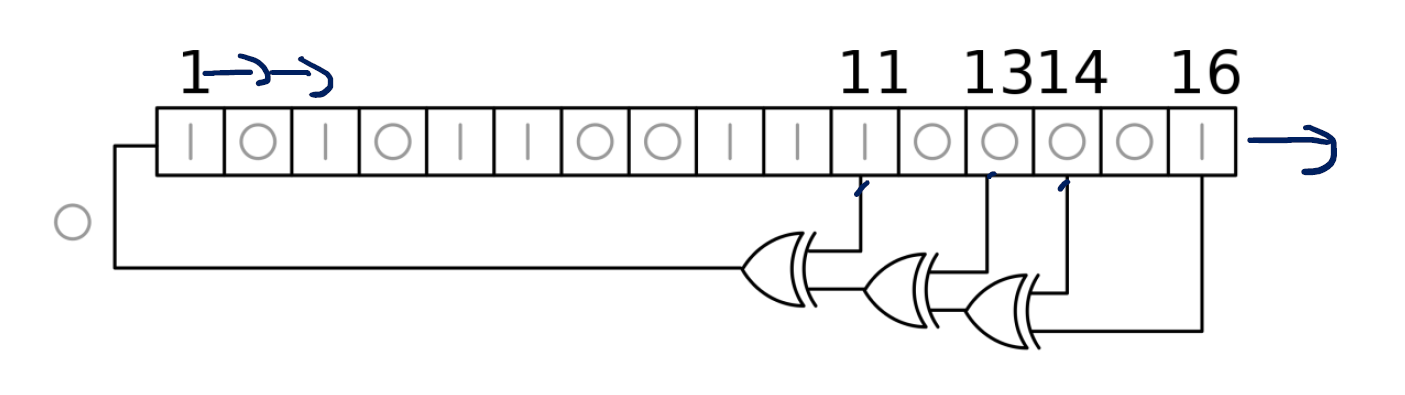
\includegraphics[width=120mm]{Graphics/Basics of Private Key Encryption/PseudorandomnessagainstSimpleStatisticalTests.png}\newline
		\end{center}
	
	\begin{definition}[Pseudorandom Generators]\ 
	    \begin{itemize}
	        \item $G(K)$: deterministic polynomial time algorithm, takes as input $K \in \{0,1\}^{\lambda}$ and outputs $G(K) \in \{0,1\}^l$, where $l = poly(\lambda)$.
	        \item $u$ is uniformly distributed over $\{0,1\}^l$
	        \item A distinguisher is an algorithm which outputs a single bit.
	        \item $G$ is a pseudorandom generator, if it holds for every PPT distinguisher $\mathcal{D}$ that
	            \begin{itemize}
	                \item $\vert Pr[\mathcal{D}(G(k))=1]-Pr[\mathcal{D}(u)=1] \vert \leq negl(\lambda)$
	                \item where probability is over $K \leftarrow \{0,1\}^{\lambda}$, $u \leftarrow \{0,1\}^l$ and the random coins of $\mathcal{D}$.\newline
	            \end{itemize}
	    \end{itemize}
	\end{definition}
	
	\section{Examples}
		\begin{itemize}
			\item Modular Congruence generator:
				\begin{itemize}
					\item $P$ a prime
					\item $\mathbb{Z}_P = \{0,...,P-1\}$
					\item $a,b \leftarrow_{\$} \mathbb{Z}_P$
					\item $x_0 \leftarrow_{\$} \mathbb{Z}_P$
					\item $s = (a,b,x_0)$
					\item $G(s):$ Compute a sequence $x_0,x_1,...,x_l$ via $x_{i+1} \leftarrow a \cdot x_i + b\ mod\ P$
				\end{itemize}
			\item Is this a pseudorandom generator?
				\begin{itemize}
					\item No!
					\item Sequence in completely determined by $x_0,x_1,x_2$
						$$a = \frac{x_2-x_1}{x_1-x_0}\ mod\ P \text{,}\ b = x_1 -a \cdot x_0\ mod\ P$$
						$$x_1 = a \cdot x_0 + b\ mod\ P$$
						$$x_2 = a \cdot x_1 + b\ mod\ P$$
					\item \textbf{Distinguishing attack:} Compute $a,b$ from $x_0,x_1,x_2$ and test for all $i > 2$ if $x_i = a \cdot x_{i-1} + b\ mod\ P$
					\item For a uniform sequence this happens only with probability $P^{-(l-3)}$
					\item Distinguishing advantage: $1-P^{-(l-3)}$
				\end{itemize}
		\end{itemize}
	
	
	\begin{theorem}[Security of Stream Ciphers]\ \\
	    If $G$ is a pseudorandom generator, then $(KeyGen,Enc,Dec)$ is $IND$-secure.
	\end{theorem}
	\begin{proof}
		\textit{Proof by Contraposition:}\\
		Assume $(KeyGen,Enc,Dec)$ is not $IND$-secure\\
		$\Rightarrow$ There is at least one PPT $\mathcal{A}$ and a non-negligible $\epsilon$ so that
		$$Pr[IND_{\mathcal{A}}(\lambda) = 1] = \frac{1}{2} + \epsilon$$
		\begin{center}
			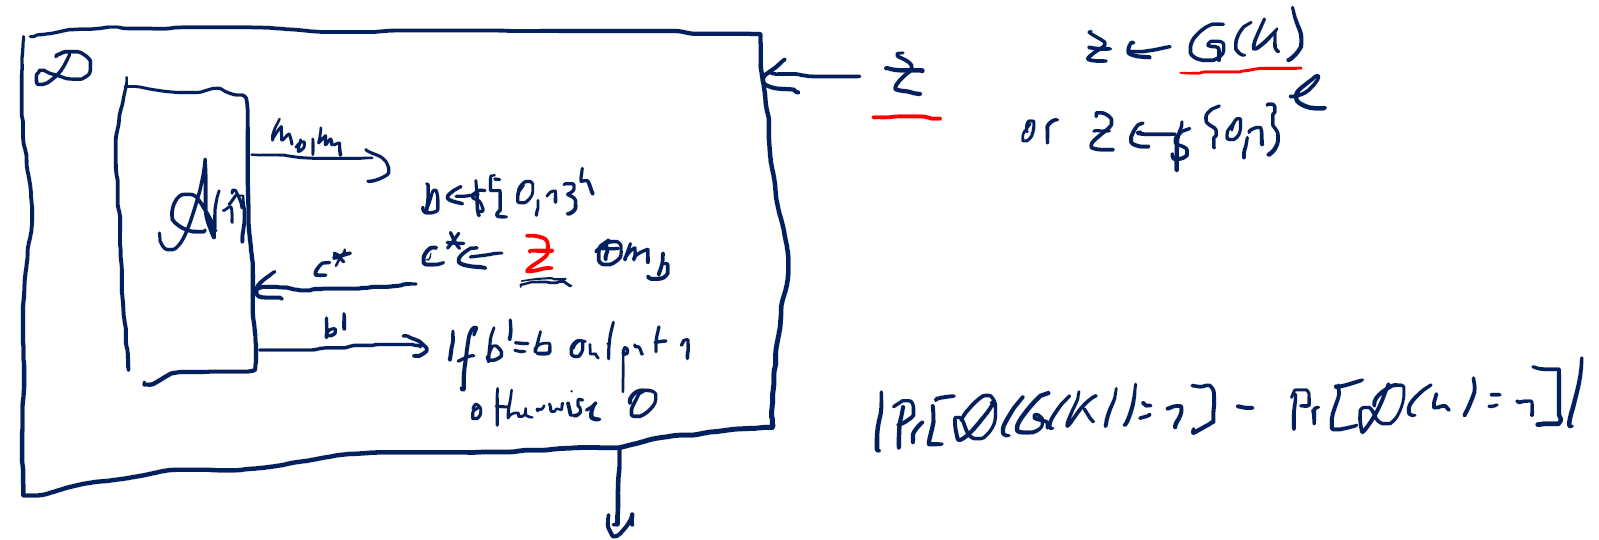
\includegraphics[width=160mm]{Graphics/Stream Ciphers/thm4_1.png}\newline
		\end{center}
		$$Pr[\mathcal{D}(G(K)) = 1] = Pr[IND_{\mathcal{A}}(\lambda) = 1] = \frac{1}{2} + \epsilon$$
		But $Pr[\mathcal{D}(u) = 1] = \frac{1}{2}$ and so it follows, that\\
		$$|Pr[\mathcal{D}(G(K)) = 1] - Pr[\mathcal{D}(u) = 1]| = \frac{1}{2} + \epsilon - \frac{1}{2} = \epsilon$$
		is non-negligible. Therefore $G$ is not a PRG and so the theorem is proven.
	\end{proof}
	
\section{Summary}
	\begin{itemize}
		\item Cryptographic pseudorandom generators (PRGs) need to fool all statistical tests, not just a few we chose
		\item Pseudorandom Generators generate distributions that are far from uniform but cannot be distinguished from uniform by any PPT algorithm
		\item PRGs imply IND secure stream ciphers, for which the key is shorter than the message
	\end{itemize}

	



































